\chapter{Dynamo}
\label{Dynamo}


\section{Problemstellung und Einordnung}
Amazon wickelt Bestellungen von Kunden rund um die Welt ab. Hierfür benötigt Amazon ein hochverfügbares System, das sicherstellt, dass jederzeit Bestellungen entgegen genommen werden können. Es werden also viele Rechenzentren benötigt, um diese Last zu tragen. Bei der Auswahl von Rechnern für diese Rechenzentren setzt Amazon allerdings nicht auf hochverfügbare Spezialhardware, sondern setzt handelsübliche Rechner ein. Um dennoch eine möglichst hohe Verfügbarkeit garantieren zu können, hat Amazon die verteilte Datenbank Dynamo entwickelt, die in \cite{dynamo} beschrieben wurde und in diesem Kapitel vorgestellt werden soll. \\ 
\\
Dynamo ist dafür konzipiert, bei Verfügbarkeit einer minimalen Anzahl an Knoten, Schreibvorgänge annehmen zu können. Dynamo ist also partitionierungstolerant und hoch verfügbar, kann Datenkonsistenz aber nur unter bestimmten Bedingungen garantieren. 
\section{Datenmodell}
Dynamo ist ein Key-Value-Store. Werte werden also unter einem Schlüssel abgelegt und können nur über diesen Schlüssel wieder abgefragt werden. Komplexere Anfragen sind daher nicht möglich. Der Wert, der hinterlegt wird, muss keinem festen Datenschema entsprechen - es können beliebige Binärdaten gespeichert werden.

\section{Architektur}

\subsection{Konsistentes Hashing}
Um die Daten den Knoten zuzuordnen, verwendet Dynamo konsistentes Hashing. Hierbei wird für jeden Schlüssel ein MD5 128 Bit Hash-Wert gebildet. Den Knoten wird ebenfalls ein Wert zwischen $0$ und $2^{128}$ zugeordnet. Ein Schlüssel-Wert-Paar wird auf dem Knoten gespeichert, dem der nächst höhere Wert ausgehend vom Hash-Wert des Schlüssels zugeordnet wurde. Gibt es keinen Knoten, der einen höheren Wert hat, wird das Schlüssel-Wert-Paar auf dem Knoten mit dem kleinsten Wert gespeichert.\\
Visuell lässt sich dieses Verfahren wie in Abbildung \ref{fig:bspKonHash} mithilfe eines Kreises darstellen. Jeder Position auf dem Kreis wird im Uhrzeigersinn beginnend am obersten Punkt des Kreises ein Wert von $0$ bis $2^{128}$ zugeordnet. Knoten wie Schlüssel können dann anhand ihres Hash-Wertes auf dem Kreis platziert werden. Ein Schlüssel-Wert-Paar wird auf dem Knoten gespeichert, der auf dem Kreis an der nächsten Stelle im Uhrzeigersinn liegt.
\begin{figure}
	\caption{Beispiel für konsistentes Hashing. Die Daten sollen auf vier Knoten verteilt werden, wobei die Knoten gleichmäßig auf dem Kreis platziert sind.}
	\label{fig:bspKonHash}
	\centering
	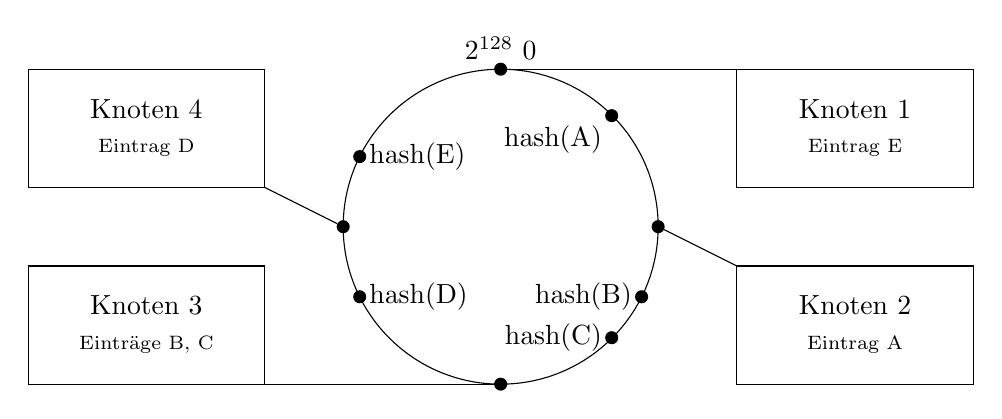
\begin{tikzpicture}
		\draw (0,0) circle (2cm);
		\node[fill=black,circle,scale=0.5] (zero) at (0,2) {};
		\node[above] at (zero) {$2^{128}$ $0$};
		\node[fill=black,circle,scale=0.5] (A) at (1.41,1.41) {};
		\node[below left] at (A) {hash(A)};
		\node[fill=black,circle,scale=0.5] (K2) at (2,0) {};
		\node[fill=black,circle,scale=0.5] (B) at (1.79,-0.89) {};
		\node[left] at (B) {hash(B)};
		\node[fill=black,circle,scale=0.5] (C) at (1.41,-1.41) {};
		\node[left] at (C) {hash(C)};
		\node[fill=black,circle,scale=0.5] (K3) at (0,-2) {};
		\node[fill=black,circle,scale=0.5] (D) at (-1.79,-0.89) {};
		\node[right] at (D) {hash(D)};
		\node[fill=black,circle,scale=0.5] (K4) at (-2,0) {};
		\node[fill=black,circle,scale=0.5] (E) at (-1.79,0.89) {};
		\node[right] at (E) {hash(E)};
		\draw (3,2) rectangle (6,0.5);
		\draw (3,-2) rectangle (6,-0.5);
		\draw (-3,2) rectangle (-6,0.5);
		\draw (-3,-2) rectangle (-6,-0.5);
		\draw (zero) -- (3,2);
		\draw (K2) -- (3,-0.5);
		\draw (K3) -- (-3,-2);
		\draw (K4) -- (-3,0.5);
		\node at (4.5,1.5) {Knoten 1};
		\node at (4.5,1) {\scriptsize{Eintrag E}};
		\node at (4.5,-1) {Knoten 2};
		\node at (4.5,-1.5) {\scriptsize{Eintrag A}};
		\node at (-4.5,-1) {Knoten 3};
		\node at (-4.5,-1.5) {\scriptsize{Einträge B, C}};
		\node at (-4.5,1.5) {Knoten 4};
		\node at (-4.5,1) {\scriptsize{Eintrag D}};
	\end{tikzpicture}
\end{figure}
\subsection{Replikation}
Replikation lässt sich nun leicht realisieren, indem die Einträge nicht nur auf dem nächsten, sondern bei einem Replikationsfaktor von $n$ auf den nächsten $n$ Knoten gespeichert werden. Fällt dann ein Knoten aus, lassen sich die Einträge weiterhin auf dem jeweils nächsten Knoten auf dem Kreis auffinden. Bei einem Ausfall muss dafür gesorgt werden, dass die Bedingung, dass alle Daten auf den nächsten $n$ Knoten gespeichert sind, wieder hergestellt wird.
\subsection{Partitionierung und Verteilung}
Bei der Partitionierung aus Abbildung \ref{fig:bspKonHash} ist beim Ausfall eines Knotens das Problem, dass die nächsten $n$ Knoten (bei Replikationsfaktor $n$) die volle Last das Ausfalls tragen müssen, da die Daten, die der ausgefallene Knoten gespeichert hat, auf die nächsten $n$ Knoten repliziert werden müssen. Ist $n$ im Vergleich zur Anzahl der insgesamt verfügbaren Knoten eher klein, wäre es wünschenswert eine bessere Verteilung der Last zu erzielen. Daher platziert Dynamo die Knoten nicht direkt auf dem Kreis, sondern plaziert stattdessen virtuelle Knoten. Dabei stehen mehrere virtuelle Knoten für einen realen Knoten. Nun können die virtuellen Knoten so auf dem Kreis verteilt werden, dass auf die virtuellen Knoten eines realen Knotens die virtuellen Knoten verschiedener realer Knoten folgen. Bei dem Ausfall eines realen Knotens wird die entstehende Last also auf viele oder sogar alle realen Knoten verteilt.\\
\\
In Abbildung \ref{fig:bspKonHash} wurden die Knoten gleichmäßig auf dem Kreis verteilt. Es ließe sich nun ein Schema finden, das für virtuelle Knoten eine Verteilung auf dem Kreis bestimmt, durch die die virtuellen Knoten ebenfalls gleichmäßig auf dem Kreis verteilt werden, und dafür sorgt, dass der Ausfall eines Knotens zunächst von allen anderen Knoten getragen wird. Das Problem ist jedoch, dass das Schema nach dem Ausfall erneut ausgeführt werden müsste, um eine gleichmäßige Verteilung wieder herzustellen. Hierbei würden jedoch meist alle virtuellen Knoten neu platziert werden und es müssten viele Daten verschoben werden. Ein ähnliches Szenario würde das Hinzufügen eines Knotens hervorrufen.\\
Da der Aufwand für das Verschieben der Daten zu hoch wäre, lässt sich ein solches optimales globales Schema nicht realisieren. Stattdessen wurden von Amazon drei Strategien zur Verteilung der Daten evaluiert. Diese werden im Folgenden vorgestellt:
\subsubsection*{Strategie 1}
Die erste Strategie verteilt die virtuellen Knoten zufällig auf dem Kreis. Hierdurch lässt sich eine gute Lastverteilung bewirken, da es unwahrscheinlich ist, dass ein Knoten im Vergleich zu den anderen Knoten einen sehr viel größeren Bereich des Kreises zugewiesen bekommt. Des Weiteren ist die Wahrscheinlichkeit gering, dass auf die meisten virtuellen Knoten eines realen Knotens fast ausschließlich virtuelle Knoten eines einzigen anderen realen Knotens folgen.\\
Außerdem hat diese Strategie den Vorteil, dass das Hinzufügen eines neuen Knotens eine verteilte Operation ist: Der Knoten kann die Positionen seiner virtuellen Knoten zufällig auswählen und die realen Knoten, die die Daten seines Bereichs halten, um die Übergabe der Daten bitten. Diese Knoten können dann ihren Speicher nach Einträgen durchsuchen, die übergeben werden sollen.\\
Es wurde jedoch festgestellt, dass eben dieses Durchsuchen des Speichers eines Knotens sehr aufwändig ist, da alle Einträge überprüft werden müssen. Strategie 2 vereinfacht diesen Suchvorgang. 
\subsubsection*{Strategie 2}
Strategie 2 wurde nur für kurze Zeit eingesetzt und kann als Zwischenschritt zu Strategie 3 betrachtet werden.\\
Strategie 2 unterteilt den Kreis in gleichgroße Partitionen. Dabei muss die Anzahl der Partitionen sehr viel größer sein als die Anzahl der potentiellen virtuellen Knoten. Ein Knoten speichert immer nur die Daten einer vollen Partition. Auch Strategie 2 verteilt die virtuellen Knoten zufällig auf dem Kreis. Auf die gleiche Weise, wie bei Strategie 1 die Einträge auf die Knoten zugeordnet wurden, werden bei dieser Strategie die Partitionen den Knoten zugeordnet. Ein Knoten legt einen neuen Eintrag dann im Speicherbereich der entsprechenden Partition ab. Wird er von einem neuen Knoten aufgefordert, einen Bereich des Kreises abzugeben, muss er nicht seinen kompletten Speicher nach Einträgen durchsuchen, sondern nur die zum Bereich gehörenden Partitionen bestimmen. Hierdurch wird nicht nur der Suchaufwand beim Hinzufügen eines Knotens verringert, sondern auch der benötigte Speicher, um festzuhalten, welcher Bereich des Kreises auf welchem Knoten liegt, verringert sich immens.
\subsubsection*{Strategie 3}
Strategie 3 geht wie Strategie 2 vor, bis auf dass die Knoten nicht mehr auf dem Kreis platziert werden, sondern die Partitionen den Knoten direkt zufällig zugeordnet werden. Kommt ein neuer Knoten hinzu, erhält er von jedem Knoten die gleiche Anzahl an zufällig ausgewählten Partitionen.
\subsection{Die put()- und die get()-Operation}
Mit der put()-Operation lassen sich Daten in Dynamo anlegen. Wird die put()-Operation an einem Knoten aufgerufen, informiert dieser Knoten zunächst den nächsten erreichbaren Knoten auf dem Kreis ausgehend vom Hash-Wert des Schlüssels des neuen Eintrags. Dieser Knoten ist für das weitere Verfahren verantwortlich. Hat er die Nachricht erhalten, speichert er den Eintrag und informiert die nächsten $N-1$ Knoten auf dem Kreis über den Eintrag. Hat er von $W-1$ Knoten eine Bestätigung erhalten, dass diese den Eintrag ebenfalls gespeichert haben, kann er den Nutzer informieren, dass der Eintrag gespeichert ist. Der Nutzer erhält die Bestätigung also, wenn der Eintrag auf $W$ Knoten abgelegt ist. Anschließend wartet der verantwortliche Knoten, ob er von den restlichen Knoten eine Antwort bekommt und informiert den nächsten Knoten auf dem Kreis ebenfalls über den Eintrag, falls einer der $N-1$ Knoten nicht reagiert. Das Ziel ist also, den Eintrag $N$ Mal zu speichern. \\
Bei der get()-Operation wird die Anfrage ebenfalls zunächst an den verantwortlichen Knoten übermittelt. Dieser leitet die Anfrage an $N-1$ Knoten weiter und beantwortet die Anfrage, wenn ihm die Ergebnisse von $N-1$ anderen Knoten und sein eigenes Ergebnis zur Verfügung stehen. Um Widersprüche in den Ergebnissen auflösen zu können, wird eine Versionierung der Daten benötigt.
\subsection{Versionierung}
Dynamo verändert gespeicherte Einträge nicht, sondern behandelt eine Änderung als neue Version der Daten. Dynamo verwendet Vektoruhren, um aufzulösen, welche Version eines Eintrages neuer ist. Der Zeitstempel des alten Eintrages wird bei einem Update vom Nutzer der Datenbank mitgegeben, sodass der Knoten, der für den neuen Eintrag verantwortlich ist, einen neuen Zeitstempel erstellen kann. Findet ein Knoten zwei Einträge vor, die widersprüchliche Vektoren haben, also keine Aussage getroffen werden kann, welcher Eintrag neuer ist, speichert er beide Einträge ab und bei der nächsten Anfrage werden beide Einträge dem Nutzer übergeben. Dieser muss dann den Konflikt auflösen. \\
\\
Es gibt einige Anwendungsfälle, in denen eine solche Konfliktlösung leicht ableitbar ist. So wird in \cite{dynamo} der Anwendungsfall des virtuellen Einkaufskorbs als Beispiel genannt. Hatte ein Nutzer die Version 1 seines Einkaufkorbes und hat anschließend zwei Artikel in den Einkaufskorb gelegt, wobei beim ersten Artikel basierend auf Version 1 eine Version 2 des Einkaufskorbes erstellt wurde und beim zweiten Artikel ebenfalls basierend auf Version 1 eine Version 3 erstellt wurde, so lässt sich der Konflikt zwischen Version 2 und Version 3 leicht durch das Vereinigen der beiden Einkaufskörbe lösen. Auf diese Weise kann kein hinzugefügter Artikel verloren gehen. Nur wenn ein Artikel entfernt wurde, kann es dazu kommen, dass dieser Artikel wieder im Einkaufskorb landet.
\section{Erneute Einordnung}
Mithilfe der Parameter $W$ und $R$ kann Dynamo etwas differenzierter im CAP-Theorem eingeordnet werden. Je niedriger die Parameter $W$ und $R$ sind, desto verfügbarer und partionierungstoleranter wird Dynamo. Werden beide Parameter auf $1$ gesetzt, reicht ein verfügbarer Knoten, um eine Schreiboperation durchzuführen und ein verfügbarer Knoten, der eine beliebige Version des Eintrag gespeichert hat, um eine Anfrage zu beantworten. Allerdings leidet die Konsistenz unter sehr niedrigen Werten $W$ und $R$. Werden $W$ und $R$ auf die Anzahl der Knoten gesetzt, ist Dynamo komplett konsistent, aber weder verfügbar, wenn ein Knoten ausfällt, noch partitionierungstolerant.